% 6.4 Discussion
\subsection{Discussion}
% Hard to assess 3d seg from 2d image
% Compare differences at each number
A visual example of the findings from the size distribution
assessment is provided for the different segmentations of the
Kel-F - F50 sand system. A comparison is made between an image sliced from
the rescaled CT scan (\ref{fig/06/seg}.a) and the slice at the
corresponding location in each of the three segmentations determined to have
the lowest total accumulated error in size distribution. These segmentations
were seeded by markers selected with 5, 6, and 7 pixel minimum peak
distances and are hereafter referred to as
Segmentation B (\ref{fig/06/seg}.b), Segmentation C
(\ref{fig/06/seg}.c), and Segmentation D (\ref{fig/06/seg}.d),
respectively. Labeled sand grains of interest (\ref{fig/06/seg}.a) are
compared to corresponding segmented particles in each of these segmentations.

Across these segmentations, there is a trend of particles that are more
segmented in Segmentation B and become less segmented in Segmentation C and
Segmentation D.
There are not many over-segmented particles visible in this slice of the
volume, but the evidence over-segmentation can be seen in the segmented
representations of sand grain 3. In Segmentation B and Segmentation C this
sand grain is over-segmented as two particles. In Segmentation D, these two
regions are segmented as a single particle, but it is unclear from this
slice whether or not the sand grain to the lest is also merged into the
particle. Other sand grains are represented distinctly in Segmentation B
and Segmentation C but are erroneously under-segmented in Segmentation
D as is the case with sand grain 1 and sand grain 2 as well as sand grain 11
and sand grain X.
There are a few cases of sand grains segmented distinctly in Segmentation B
that are under-segmented in Segmentation C and Segmentation D. This occurs with
the pair of sand grains 8 and 9 as well as the group of particles 13, 14,
and 15.
Some particles are under-segmented in all three of the segmentations. This is
true of sand grains 5 and 6, which appear as a single particle in each
segmentation.
There are also certain cases in which sand grains that segmented distinctly in
Segmentation B appear to be un-segmented from surrounding binder material as
is the case with sand grains 4 and 12.
and what appears to be some of the surrounding binder material.
The final class of particles that appear here are particles in Segmentation B,
but are too small and close to other markers to appear in Segmentation C and
Segmentation D due to the minimum distance of the markers chosen to seed
these segmentations. This can be seen with sand grain 7.

All these examples show more under-segmented particles in Segmentation D
than in Segmentation B and Segmentation C, though Segmentation
B does have some under-segmented particles that appear to be properly
segmented in Segmentation B. Regardless, Segmentation B and Segmentation C
were both shown to minimize the
lowest total accumulated error in the two size distribution analyses in part
because the error was spread across the mean size of typically distributed
particles, with some smaller particles as well as some larger particles.
The other segmentations which resulted in higher total accumulated error
mainly had particles that were either majority smaller or majority larger
than the mean of the typical distribution.
The fact that Segmentation C had the lowest total accumulated error suggests
that the number of under-segmented particles balances out the over-segmented
particles that are also shown to be present.

% 3        over  over  well
% 1-2      well  well  under
% 4        well  well  under
% 12       well  under under
% 11       well  under under
% 8-9      well  under under
% 13-14-15 well  under under
% 5-6      under under under
% 7        well  xx    xx
% 10       well  well  well

\begin{figure}[ht]
    \centering
    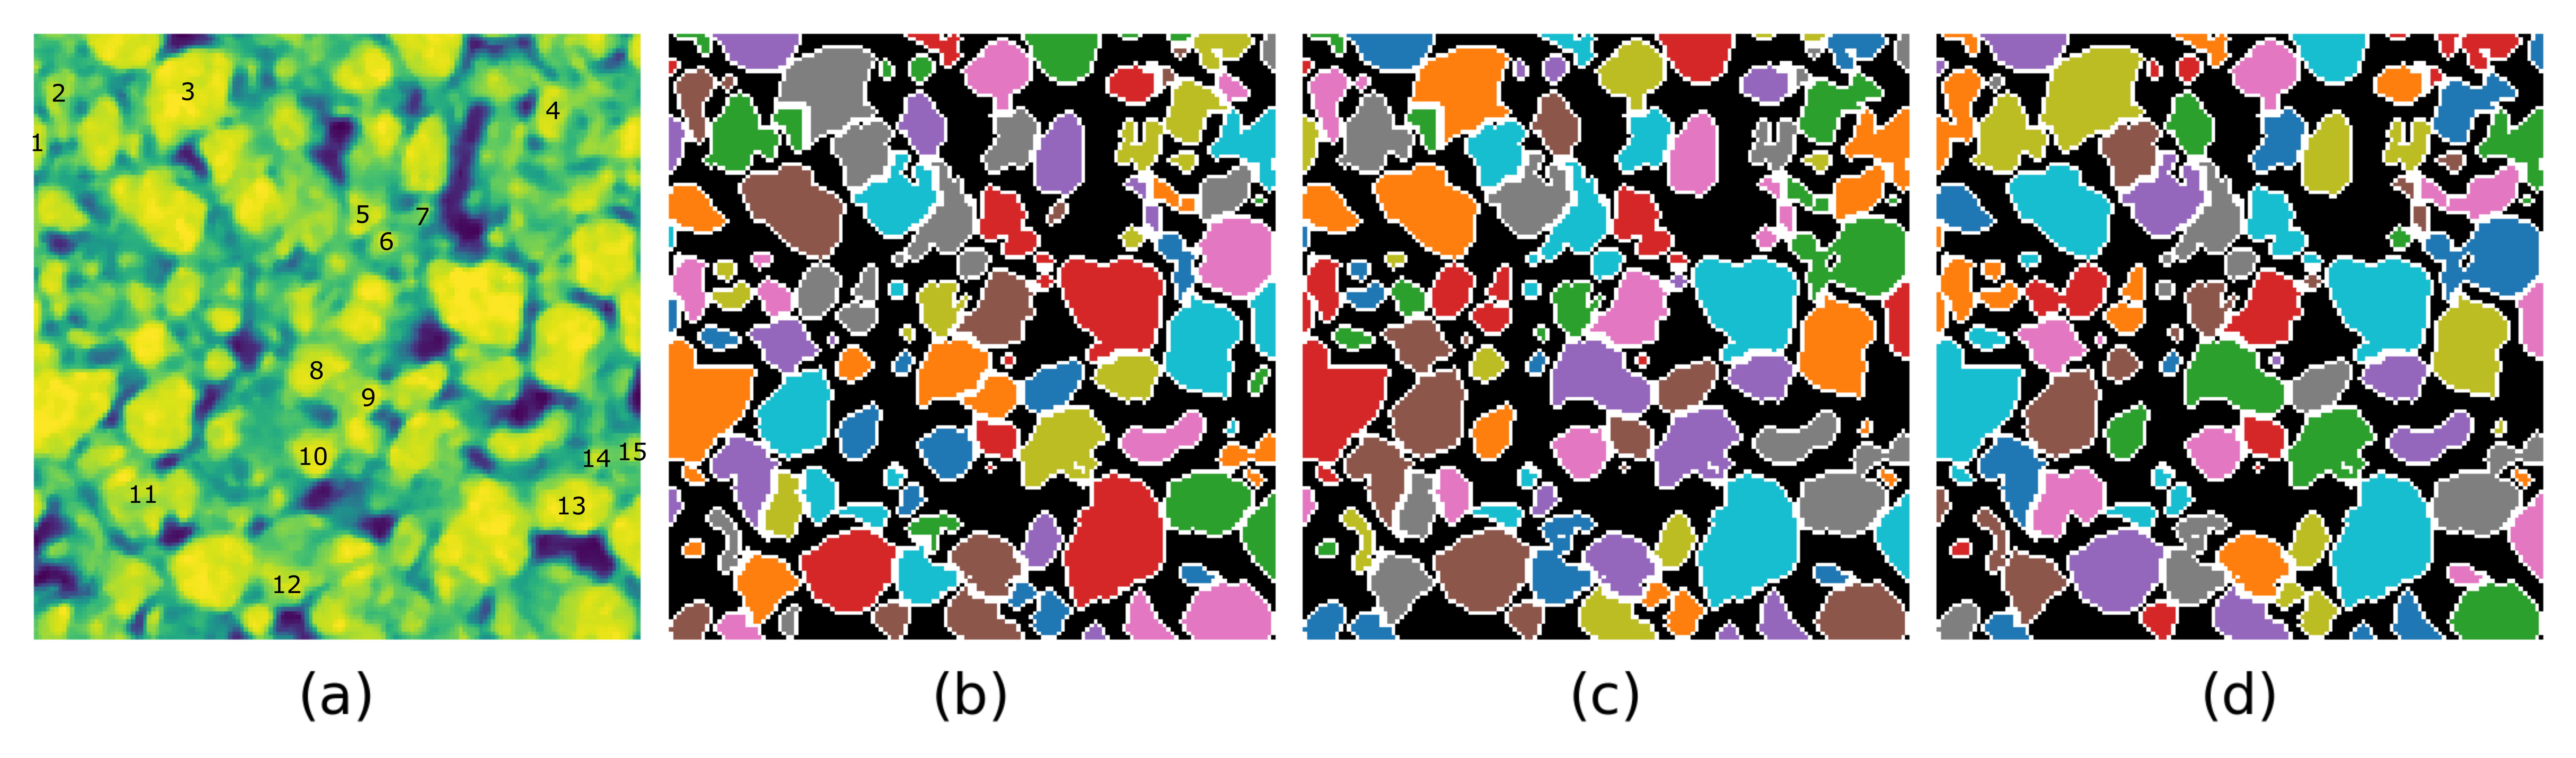
\includegraphics[width=0.9\textwidth]{figures/06/08-slice_525-full_seg-5-6-7.png}
    \caption{
        \small\setstretch{1}
        (a) A slice of the rescaled intensity CT scan image with particles of
        interest labeled to allow for ease of comparison and discussion
        between the three segmentations.
        (b) Corresponding slice of Segmentation B, as seeded by markers
        selected with a 5 pixel minimum peak distance, with the second lowest
        total accumulated error in particle size.
        (c) Corresponding slice of Segmentation C, as seeded by markers
        selected with a 6 pixel minimum peak distance, with the lowest
        total accumulated error in particle size.
        (d) Corresponding slice of Segmentation D, as seeded by markers
        selected with a 7 pixel minimum peak distance, with the third lowest
        total accumulated error in particle size.
    }
    \label{fig/06/seg}
\end{figure}

It is interesting that the watershed segmentation that performed the best was
seeded with markers determined with a 6 pixel minimum peak distance. This
correlates to a physical distance of 83.04 µm between markers,
which is between the second and
third smallest mesh sizes used to assess the particle sizes.
The 4 pixel minimum peak distance, which corresponds most closely to the
smallest mesh size (53 µm) at a physical distance of 55.36 µm, did not
produce results that aligned well with the typical size distribution, with
a total error among the highest of the tested segmentations. At a first glance,
this is unexpected, as one might expect the minimum space between markers to
be small enough to allow all the smallest particles to be segmented. However,
this result shows that it is actually more important to choose a larger
minimum peak distance to achieve a size distribution that is more
representative of reality. As can be seen in the left-shifted cumulative size
distributions of the 4 pixel minimum peak distance segmentation, the majority
of particles are smaller than typical F50 particles.
This means that generating markers based on a
distance that is closer to the size of the smallest particles results in
particles are over-segmented.
In contrast, the best fitting 5 and 6 pixel minimum peak distance segmentations
are distributed among each side of the typical F50 distribution, suggesting
a balance of over- and under-segmentation.

To demonstrate the mesh postprocessing capabilities of \textit{Segmentflow},
the surface mesh generated from the segmented particle corresponding to sand
grain 10 (\ref{fig/06/seg}.a) is shown independently and compared with
the meshes resulting varying amounts of postprocessing. The surface mesh
as-computed by the marching cubes algorithm is made up of 1524 triangles
(\ref{fig/06/postprocess}.a). After Laplacian smoothing, the mesh
retains the same number of triangles, but the result appears less blocky
(\ref{fig/06/postprocess}.b). The mesh is also shown after
simplification past 200 triangles, resulting in mesh made up of 190 triangles
(\ref{fig/06/postprocess}.c). The final mesh shows extreme
simplification past 20 triangles to a resulting mesh of only 10 triangles
(\ref{fig/06/postprocess}.d). This ability to tune the complexity of
the surfaces of each segmented particle is referred to as the
``exascale knob'' as it allows the user to determine the complexity of the
simulation which will use the resulting geometry.

\begin{figure}[ht]
    \centering
    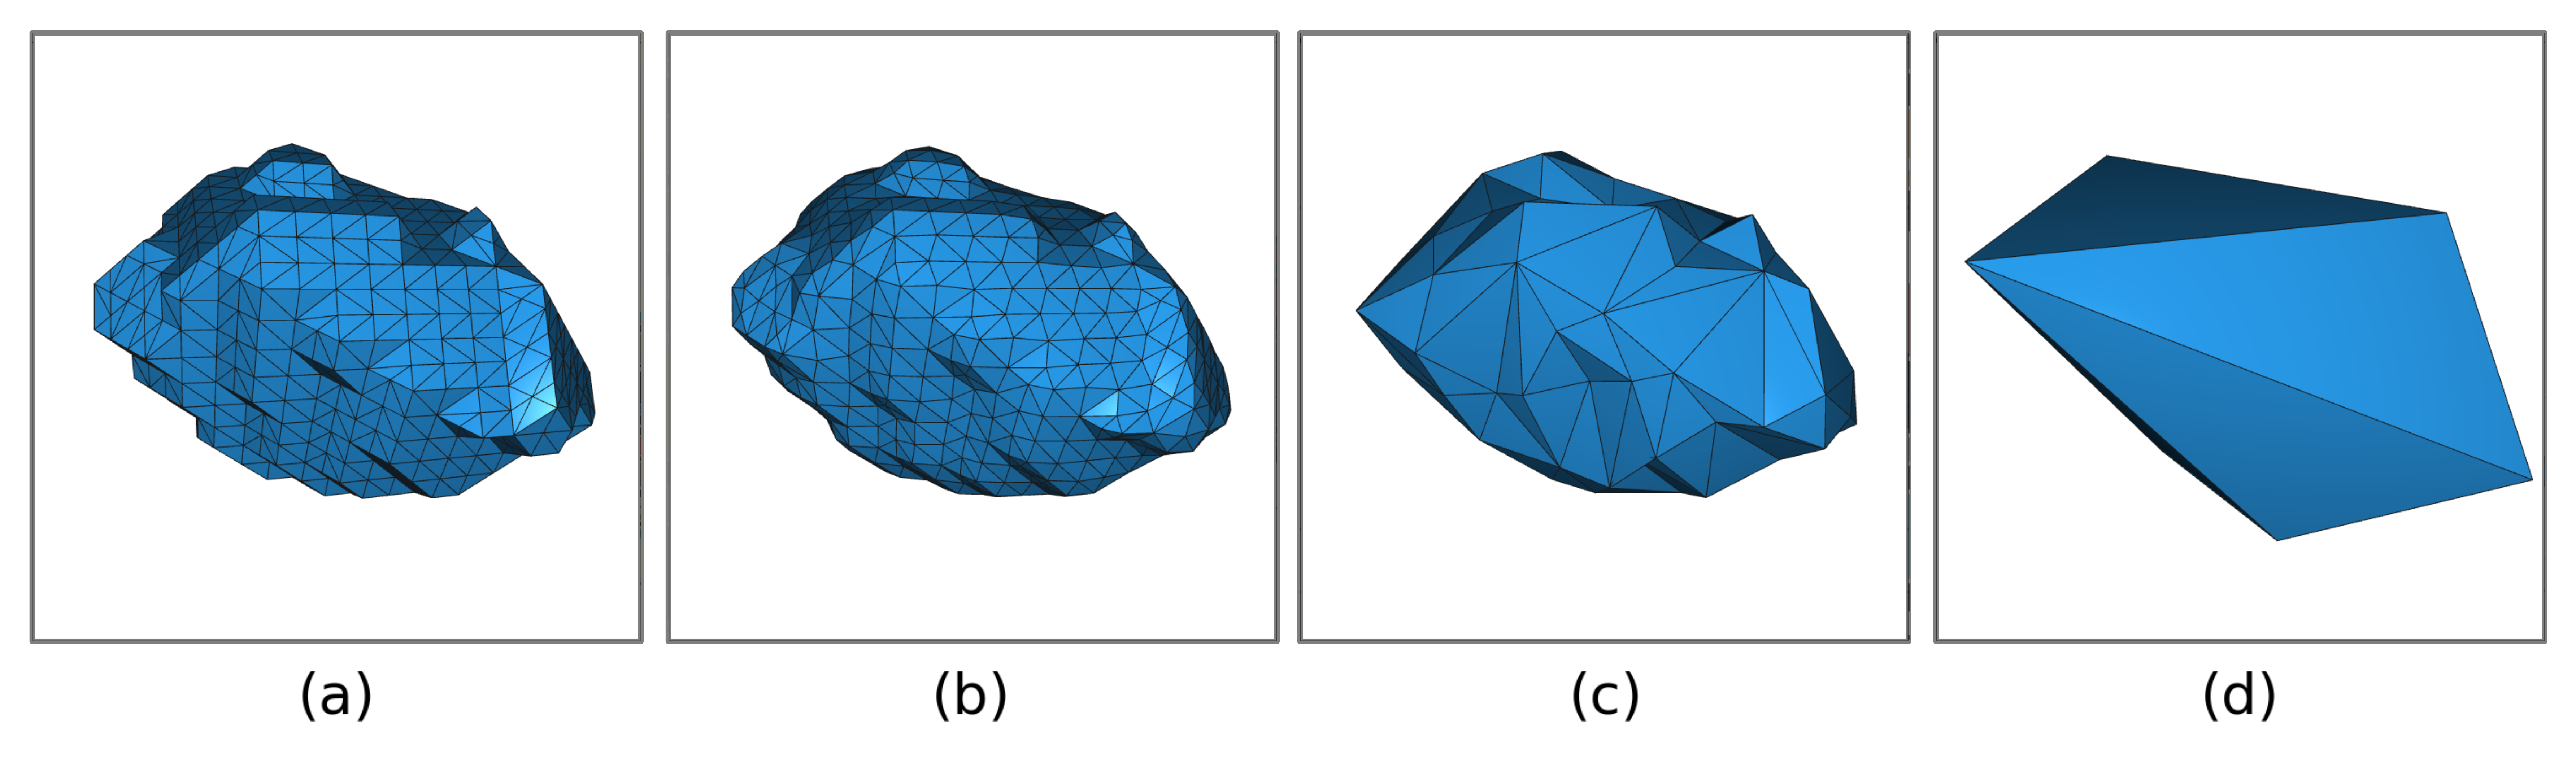
\includegraphics[width=0.9\textwidth]{figures/06/06-26259-mesh-tris-1524-190-10.png}
    \caption{
        \small\setstretch{1}
        (a) Surface mesh produced from a segmented particle. Mesh originally
        has 1524 triangles across its surface.
        (b) Smoothing applied to surface mesh as part of the mesh
        postprocessing capabilities of \textit{Segmentflow}.
        (c) Mesh simplified beyond 200 triangles.
        (d) Mesh simplified beyond 20 triangles.
    }
    \label{fig/06/postprocess}
\end{figure}

